\section{The Ionosphere}
The ionosphere, extending from $\approx$ 85 km to 1000 km, is the highly-variable transition region between the terrestrial neutral atmosphere and the sparse plasmas of the space environment. The relatively-sharp rise in electron density at the bottom of the ionosphere makes it highly-reflective within the VLF band, forming a waveguide between it and the conductive surface of the Earth. However, In studying LEP, we are primarily concerned with the fraction of energy which does not reflect, and instead propagates through the ionosphere and out into the plasmasphere.

\subsection{Trans-Ionosphere Attenuation}
\label{section:trans_ionosphere_atten}
The ionosphere is a region of high variability, and a significant factor in the LEP process. As discussed earlier, the majority of VLF energy emitted by a lightning flash propagates efficiently in the Earth-Ionosphere waveguide; however a fraction of emitted energy can propagate upwards through the ionosphere, where the wave experiences significant losses via Joule heating in the D-region ionosphere \citep{Graf2013, Blaes2016}.

Propagation through the ionosphere is ill-suited for a raytracing approach, as in section \ref{section:raytracing}, for several reasons: first, the ionosphere electron density varies significantly across a relatively thin slab, effectively violating the WKB (smoothly-varying) approximation. Second, the Landau calculations used to compute ray damping are designed for warm, but collisionless plasmas; the ionosphere is collisional, and only partially ionized, requiring different treatment.

Ionospheric propagation is further complicated by reflection and transmission at the lower boundary layer, as well as mode-coupling between incident plane waves, the whistler mode, and various others. 

For computational simplicity, and to more-easily generalize to a variety of conditions, we treat the ionosphere as a single absorbing slab, ranging from 100 to 1000 km in altitude. We assume that waves propagate directly upwards (normal to the Earth's surface), and are not deflected by ionospheric irregularities or the inclination of the background magnetic field.

Numerous researchers \citep{Lauben1998, Bortnik2005, Kulkarni2009, Graf2013} have used the classic ``Helliwell" curves, taken from \cite{Helliwell1965}, figure 3-35. Helliwell performs an analysis similar to Landau damping -- first deriving a dispersion relation for a collisional plasma, then separating out the imaginary component, which will result in a real-valued attenuation term. The resulting attenuation term is dependent on electron density as a function of altitude, which was extrapolated from sounding rocket campaigns for day and night. The net attenuation is then computed by integrating from 65 to 1500 km in altitude.

Helliwell's curves have persisted as the default record of trans-ionospheric attenuation; however it has been shown that Helliwell's curves overestimate trans-ionosphere attenuation by 10 to 20 dB \citep{Starks2008}, due mainly to the coarse measurement of the ionosphere electron density profile.

Rather than Helliwell's curves, we use results from \cite{Graf2013}, which are derived from extensive full-wave simulations using the International Reference Ionosphere (IRI) plasma density profile. Related work using the same full-wave model has been experimentally verified at $\sim$20 kHz using DEMETER satellite measurements of VLF transmitters \citep{Cohen2012}. \citeauthor{Graf2013} reports a set of curves in the same manner as Helliwell -- power attenuation as a function of latitude, for two frequencies (2 kHz and 20 kHz), for dayside and nightside ionospheres. We then interpolate (or extrapolate) in log-space to find an attenuation factor for any latitude or frequency of interest ($\approx 10^\circ - 70^\circ$, and 200 Hz - 30 kHz).

We transition between the dayside and nightside attenuation curves using a Sigmoid function, with an approximate 1-hour transition width.

Figure \ref{fig:graf_curves} compares the \cite{Graf2013} and \cite{Helliwell1965} attenuation curves, which model the integrated wave power losses between 65 km - 1500 km altitude as a function of frequency and geomagnetic latitude. Both models exhibit similar trends -- higher attenuation towards the equator, and higher attenuation on the dayside -- however the Helliwell curves report significantly greater attenuation overall. We can attribute this due to the electron density profile used in their calculation.

% (Also here's where you left off in incorporating Bob's edits, 1.12.2018)

\begin{figure}[h]
\begin{center}
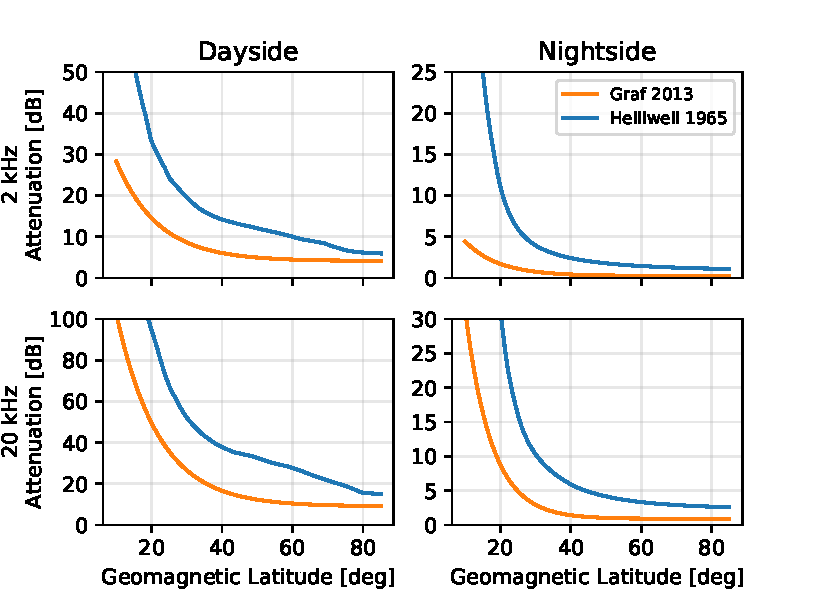
\includegraphics{figures/iono_absorp_curves}
\caption[Trans-Ionosphere attenuation curves for day and night]{Trans-Ionosphere attenuation curves for the dayside and nightside, at 2 kHz and 20 kHz. Reproduced from \cite{Graf2013}, figure 7. The \citeauthor{Graf2013} curves show markedly less attenuation than the previously-used \citeauthor{Helliwell1965} curves, especially at equatorial latitudes, and on the day side.}
\label{fig:graf_curves}
\end{center}
\end{figure}


\subsection{Models of the Ionosphere}
In general, our treatment of wave propagation in the ionosphere is abstracted using the method described in section \ref{section:trans_ionosphere_atten}. However, in raytracing through the plasmasphere, we require a smoothly-varying transition between the plasmasphere and ionosphere models. Here we discuss two models of ionosphere electron density.

\paragraph{IRI}
The International Reference Ionosphere (IRI) is a standard model of several key plasma parameters -- electron density, electron and ion temperatures, ion composition, and so forth. IRI provides detailed outputs as a function of location, altitude, and local time. The GCPM plasma model uses the IRI-2007 implementation \citep{Bilitza2008}; the simplified IRI model is derived from the IRI-2016 model (the most-current available version at time of writing).

\paragraph{Simplified IRI}
\begin{figure}[h]
\begin{center}
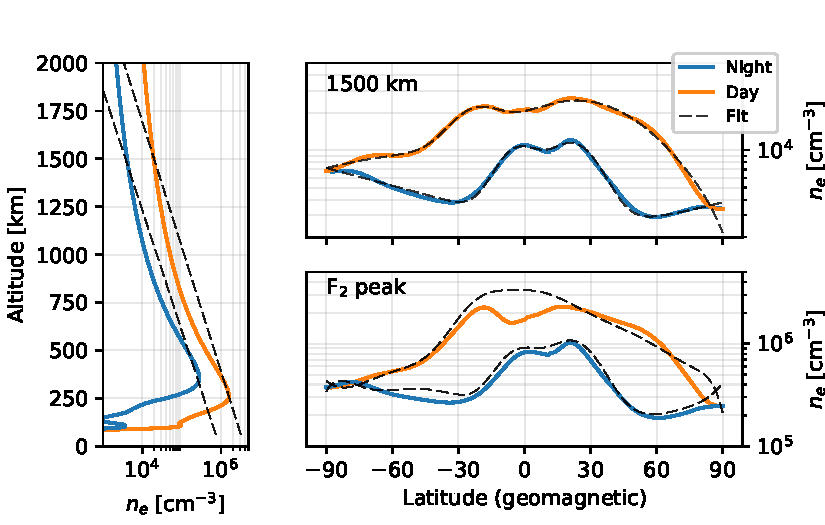
\includegraphics{figures/iono_profile.pdf}
\caption[Ionosphere density profile]{The IRI electron density model and derived curve fits. The left panel shows electron density variation as a function of altitude, for day and night. The right panels show electron density variation with respect to latitude, for (top) 1500 km and (bottom) the $F_2$ peak (approx. 300 km). Dashed lines indicate the fitted curves used by the simplified IRI model.}
\label{fig:iono_profile}
\end{center}
\end{figure}

In order to both reduce our model parameter space, and to greatly decrease computation time, we pair a simplified version of IRI with a simplified version of GCPM. The IRI-2016 model was run for dayside and nightside ionospheres (12 and 0 MLT), using all default settings, for January 1st, 2000. We then fit a multiple-Gaussian function to the electron density vs latitude, at an altitude of 1500 km, and at the $F_2$ peak. Electron density variation with respect to altitude is approximated by a log-linear fit between 1500 km and the $F_2$ peak. Finally, longitudinal variation is smoothed with a sigmoid function with a width of $\sim$ 1 hr. Figure \ref{fig:iono_profile} shows both the IRI electron density and the derived curve fits.
